\documentclass[12pt,letterpaper]{article}
\usepackage[margin=0.80in]{geometry}
\usepackage{amsmath,amssymb,booktabs,longtable,array,tabularx,enumitem,graphicx}
\usepackage[hidelinks]{hyperref}
\usepackage{lmodern}
\usepackage{fancyhdr}
\usepackage{placeins}
\usepackage{etoolbox}
\AtBeginEnvironment{tabular}{\small}
\setlength{\parindent}{0pt}
\setlength{\parskip}{0.35em}
\setlist[itemize]{leftmargin=*,nosep}
\setcounter{tocdepth}{2}
\pagestyle{fancy}
\fancyhf{}
\fancyhead[L]{Team \#00000}
\fancyhead[R]{Page \thepage}
\renewcommand{\headrulewidth}{0.4pt}
\setlength{\headheight}{15pt}

% Every canonical number is generated from results/research_model/canonical_v4.json.
% Generated by scripts/build_paper_tables.py; do not edit.
\expandafter\def\csname canonical@chicago.existing_electric\endcsname{25}
\expandafter\def\csname canonical@chicago.fleet\endcsname{1,875}
\expandafter\def\csname canonical@chicago.lifecycle_score\endcsname{--}
\expandafter\def\csname canonical@chicago.non_electric\endcsname{1,850}
\expandafter\def\csname canonical@chicago.peak_ev_deliveries\endcsname{539}
\expandafter\def\csname canonical@chicago.service_million_km\endcsname{73.08}
\expandafter\def\csname canonical@depot.Burnaby.buses\endcsname{311}
\expandafter\def\csname canonical@depot.Burnaby.mw\endcsname{15.09}
\expandafter\def\csname canonical@depot.Burnaby.ports\endcsname{269}
\expandafter\def\csname canonical@depot.Burnaby.reserve\endcsname{42}
\expandafter\def\csname canonical@depot.Hamilton.buses\endcsname{183}
\expandafter\def\csname canonical@depot.Hamilton.mw\endcsname{10.59}
\expandafter\def\csname canonical@depot.Hamilton.ports\endcsname{158}
\expandafter\def\csname canonical@depot.Hamilton.reserve\endcsname{25}
\expandafter\def\csname canonical@depot.Langley.buses\endcsname{153}
\expandafter\def\csname canonical@depot.Langley.mw\endcsname{7.17}
\expandafter\def\csname canonical@depot.Langley.ports\endcsname{132}
\expandafter\def\csname canonical@depot.Langley.reserve\endcsname{21}
\expandafter\def\csname canonical@depot.NorthShore.buses\endcsname{266}
\expandafter\def\csname canonical@depot.NorthShore.mw\endcsname{14.40}
\expandafter\def\csname canonical@depot.NorthShore.ports\endcsname{231}
\expandafter\def\csname canonical@depot.NorthShore.reserve\endcsname{35}
\expandafter\def\csname canonical@depot.PortCoquitlam.buses\endcsname{222}
\expandafter\def\csname canonical@depot.PortCoquitlam.mw\endcsname{10.08}
\expandafter\def\csname canonical@depot.PortCoquitlam.ports\endcsname{191}
\expandafter\def\csname canonical@depot.PortCoquitlam.reserve\endcsname{31}
\expandafter\def\csname canonical@depot.Richmond.buses\endcsname{167}
\expandafter\def\csname canonical@depot.Richmond.mw\endcsname{7.23}
\expandafter\def\csname canonical@depot.Richmond.ports\endcsname{144}
\expandafter\def\csname canonical@depot.Richmond.reserve\endcsname{23}
\expandafter\def\csname canonical@depot.Surrey.buses\endcsname{388}
\expandafter\def\csname canonical@depot.Surrey.mw\endcsname{16.47}
\expandafter\def\csname canonical@depot.Surrey.ports\endcsname{337}
\expandafter\def\csname canonical@depot.Surrey.reserve\endcsname{51}
\expandafter\def\csname canonical@depot.Vancouver.buses\endcsname{410}
\expandafter\def\csname canonical@depot.Vancouver.mw\endcsname{20.64}
\expandafter\def\csname canonical@depot.Vancouver.ports\endcsname{355}
\expandafter\def\csname canonical@depot.Vancouver.reserve\endcsname{55}
\expandafter\def\csname canonical@finance.agency_25_pv_billion\endcsname{5.553}
\expandafter\def\csname canonical@finance.agency_50_pv_billion\endcsname{5.301}
\expandafter\def\csname canonical@finance.baseline_gross_pv_billion\endcsname{5.247}
\expandafter\def\csname canonical@finance.economic_score_pct\endcsname{-10.63}
\expandafter\def\csname canonical@finance.plan_gross_pv_billion\endcsname{5.804}
\expandafter\def\csname canonical@lifecycle.baseline_annual_emissions_t\endcsname{40,074}
\expandafter\def\csname canonical@lifecycle.baseline_gco2e_per_service_km\endcsname{470.1}
\expandafter\def\csname canonical@lifecycle.baseline_transition_emissions_t\endcsname{400,636}
\expandafter\def\csname canonical@lifecycle.environment_score_pct\endcsname{27.53}
\expandafter\def\csname canonical@lifecycle.operation_reduction_pct\endcsname{71.93}
\expandafter\def\csname canonical@lifecycle.plan_annual_emissions_t\endcsname{29,043}
\expandafter\def\csname canonical@lifecycle.plan_gco2e_per_service_km\endcsname{340.7}
\expandafter\def\csname canonical@lifecycle.transition_emissions_t\endcsname{700,360}
\expandafter\def\csname canonical@lifecycle.transition_score_pct\endcsname{-74.81}
\expandafter\def\csname canonical@lifecycle.whole_fleet_environment_score_pct\endcsname{25.51}
\expandafter\def\csname canonical@london.existing_electric\endcsname{950}
\expandafter\def\csname canonical@london.fleet\endcsname{8,643}
\expandafter\def\csname canonical@london.lifecycle_score\endcsname{--}
\expandafter\def\csname canonical@london.non_electric\endcsname{7,693}
\expandafter\def\csname canonical@london.peak_ev_deliveries\endcsname{776}
\expandafter\def\csname canonical@london.service_million_km\endcsname{fleet case}
\expandafter\def\csname canonical@roadmap.2024.conv\endcsname{99}
\expandafter\def\csname canonical@roadmap.2024.ev\endcsname{0}
\expandafter\def\csname canonical@roadmap.2024.retire\endcsname{99}
\expandafter\def\csname canonical@roadmap.2024.stock\endcsname{5}
\expandafter\def\csname canonical@roadmap.2025.conv\endcsname{106}
\expandafter\def\csname canonical@roadmap.2025.ev\endcsname{0}
\expandafter\def\csname canonical@roadmap.2025.retire\endcsname{106}
\expandafter\def\csname canonical@roadmap.2025.stock\endcsname{5}
\expandafter\def\csname canonical@roadmap.2026.conv\endcsname{111}
\expandafter\def\csname canonical@roadmap.2026.ev\endcsname{0}
\expandafter\def\csname canonical@roadmap.2026.retire\endcsname{111}
\expandafter\def\csname canonical@roadmap.2026.stock\endcsname{5}
\expandafter\def\csname canonical@roadmap.2027.conv\endcsname{106}
\expandafter\def\csname canonical@roadmap.2027.ev\endcsname{0}
\expandafter\def\csname canonical@roadmap.2027.retire\endcsname{106}
\expandafter\def\csname canonical@roadmap.2027.stock\endcsname{5}
\expandafter\def\csname canonical@roadmap.2028.conv\endcsname{114}
\expandafter\def\csname canonical@roadmap.2028.ev\endcsname{0}
\expandafter\def\csname canonical@roadmap.2028.retire\endcsname{114}
\expandafter\def\csname canonical@roadmap.2028.stock\endcsname{5}
\expandafter\def\csname canonical@roadmap.2029.conv\endcsname{105}
\expandafter\def\csname canonical@roadmap.2029.ev\endcsname{0}
\expandafter\def\csname canonical@roadmap.2029.retire\endcsname{105}
\expandafter\def\csname canonical@roadmap.2029.stock\endcsname{5}
\expandafter\def\csname canonical@roadmap.2030.conv\endcsname{83}
\expandafter\def\csname canonical@roadmap.2030.ev\endcsname{170}
\expandafter\def\csname canonical@roadmap.2030.retire\endcsname{203}
\expandafter\def\csname canonical@roadmap.2030.stock\endcsname{175}
\expandafter\def\csname canonical@roadmap.2031.conv\endcsname{48}
\expandafter\def\csname canonical@roadmap.2031.ev\endcsname{635}
\expandafter\def\csname canonical@roadmap.2031.retire\endcsname{509}
\expandafter\def\csname canonical@roadmap.2031.stock\endcsname{805}
\expandafter\def\csname canonical@roadmap.2032.conv\endcsname{21}
\expandafter\def\csname canonical@roadmap.2032.ev\endcsname{650}
\expandafter\def\csname canonical@roadmap.2032.retire\endcsname{473}
\expandafter\def\csname canonical@roadmap.2032.stock\endcsname{1,455}
\expandafter\def\csname canonical@roadmap.2033.conv\endcsname{0}
\expandafter\def\csname canonical@roadmap.2033.ev\endcsname{645}
\expandafter\def\csname canonical@roadmap.2033.retire\endcsname{417}
\expandafter\def\csname canonical@roadmap.2033.stock\endcsname{2,100}
\expandafter\def\csname canonical@schedule.active_battery_buses\endcsname{1,817}
\expandafter\def\csname canonical@schedule.active_buses\endcsname{1,817}
\expandafter\def\csname canonical@schedule.annual_grid_gwh\endcsname{283.4}
\expandafter\def\csname canonical@schedule.annual_revenue_km\endcsname{85.24 million}
\expandafter\def\csname canonical@schedule.fleet_with_spares\endcsname{2,100}
\expandafter\def\csname canonical@schedule.non_trolley_trip_instances\endcsname{2,119,742}
\expandafter\def\csname canonical@schedule.required_peak_power_mw\endcsname{101.67}
\expandafter\def\csname canonical@schedule.reserve_buses\endcsname{283}
\expandafter\def\csname canonical@schedule.total_electric_stock\endcsname{2,375}
\expandafter\def\csname canonical@sens.central.econ\endcsname{-10.63}
\expandafter\def\csname canonical@sens.central.env\endcsname{27.53}
\expandafter\def\csname canonical@sens.central.power\endcsname{101.67}
\expandafter\def\csname canonical@sens.fossil.econ\endcsname{-10.63}
\expandafter\def\csname canonical@sens.fossil.env\endcsname{81.90}
\expandafter\def\csname canonical@sens.fossil.power\endcsname{101.67}
\expandafter\def\csname canonical@sens.newbuild.econ\endcsname{-18.34}
\expandafter\def\csname canonical@sens.newbuild.env\endcsname{9.78}
\expandafter\def\csname canonical@sens.newbuild.power\endcsname{101.67}
\expandafter\def\csname canonical@sens.slow.econ\endcsname{-13.44}
\expandafter\def\csname canonical@sens.slow.env\endcsname{22.79}
\expandafter\def\csname canonical@sens.slow.power\endcsname{85.95}
\expandafter\def\csname canonical@sens.spare10.econ\endcsname{-12.33}
\expandafter\def\csname canonical@sens.spare10.env\endcsname{29.62}
\expandafter\def\csname canonical@sens.spare10.power\endcsname{101.67}
\expandafter\def\csname canonical@sens.winter.econ\endcsname{-14.67}
\expandafter\def\csname canonical@sens.winter.env\endcsname{16.86}
\expandafter\def\csname canonical@sens.winter.power\endcsname{122.04}
\expandafter\def\csname canonical@transition.agency_25_pv_billion\endcsname{5.553}
\expandafter\def\csname canonical@transition.agency_50_economic_pct\endcsname{-4.15}
\expandafter\def\csname canonical@transition.agency_50_pv_billion\endcsname{5.301}
\expandafter\def\csname canonical@transition.baseline_gross_pv_billion\endcsname{5.247}
\expandafter\def\csname canonical@transition.economic_score_pct\endcsname{-10.63}
\expandafter\def\csname canonical@transition.peak_annual_deliveries\endcsname{650}
\expandafter\def\csname canonical@transition.plan_gross_pv_billion\endcsname{5.804}
\expandafter\def\csname canonical@transition.total_battery_purchases\endcsname{2,100}
\expandafter\def\csname canonical@vancouver.existing_electric\endcsname{280}
\expandafter\def\csname canonical@vancouver.fleet\endcsname{1,725}
\expandafter\def\csname canonical@vancouver.lifecycle_score\endcsname{27.53\%}
\expandafter\def\csname canonical@vancouver.non_electric\endcsname{1,445}
\expandafter\def\csname canonical@vancouver.peak_ev_deliveries\endcsname{650}
\expandafter\def\csname canonical@vancouver.service_million_km\endcsname{106.87}
\newcommand{\CV}[1]{\ifcsname canonical@#1\endcsname\csname canonical@#1\endcsname\else\textbf{??}\fi}

\newcommand{\unit}[1]{\mathrm{#1}}

\begin{document}

\begin{center}
Team Control Number\\
{\Large\bfseries 00000}\\[3pt]
Problem Chosen\\
{\Large\bfseries B}\\[3pt]
2023 HiMCM\\
\textbf{Summary Sheet}
\end{center}
\hrule
\vspace{0.5em}
\begin{center}
{\Large\bfseries Charging Ahead: A Service-Preserving Roadmap for an All-Electric Metro Bus Fleet}
\end{center}

\textbf{Decision problem.} Metro Vancouver can replace its fixed-route bus fleet with zero-tailpipe electric buses by 2033 while preserving the published service. Existing trolleybuses remain electric. The model chooses vehicle duties, charging requirements, depot upgrades, annual purchases and retirement dates.

\textbf{Model.} The recovered 2023 timetable contains 54,497 distinct bus trips in 25 service patterns. We assign every non-trolley trip to a compatible vehicle duty, enforce time, transfer, capacity and state-of-charge limits, and check the repeated 119-day schedule across the calendar boundary. The resulting depot-by-class packages feed a 2024--2033 integer planning model. That model selects purchases, old-bus retirements, six-year depot construction, charger capacity and the final conversion year. The recommended plan minimizes full-lifecycle emissions; discounted cost is the tie-breaker.

\textbf{Vancouver plan.} The service-feasible fleet requires \CV{schedule.fleet_with_spares} battery buses with a 15\% reserve plus the retained 275 trolleybuses. The charging schedule needs \CV{schedule.required_peak_power_mw} MW of firm depot power and \CV{schedule.annual_grid_gwh} GWh of annual electricity. The plan delivers \CV{transition.total_battery_purchases} battery buses in four annual blocks, beginning at a maximum of 650 vehicles per year. Retrofitting the six existing depots, with additional capacity only where required, is the main infrastructure pathway.

\textbf{Results.} Full-lifecycle annualized emissions fall by \CV{lifecycle.environment_score_pct}\% relative to continued low-carbon bus renewal. The 2033 operating inventory falls by \CV{lifecycle.operation_reduction_pct}\% relative to the same service under the baseline fuel mix. The ten-year gross resource cost is CAD \CV{transition.plan_gross_pv_billion} billion, compared with CAD \CV{transition.baseline_gross_pv_billion} billion for normal renewal. With 25\% and 50\% capital support, the agency's discounted cost is CAD \CV{transition.agency_25_pv_billion} billion and CAD \CV{transition.agency_50_pv_billion} billion. The separate transition ledger records \CV{lifecycle.transition_emissions_t} tonnes of near-term embodied and operating emissions.

\textbf{Whole-fleet check.} Adding unchanged trolley activity to both sides gives a full-life environmental reduction of \CV{lifecycle.whole_fleet_environment_score_pct}\%.

\textbf{Recommendation.} Start depot interconnection and design work in 2024, procure against released charging capacity, and convert standard and articulated routes first. Release double-deck and community-shuttle orders behind terminal charging and winter tests. The 50\% funding case is the recommended implementation route; without it, the conversion imposes a material public-financing burden but remains service-feasible.

\textbf{Keywords:} electric bus; service preservation; vehicle scheduling; mixed-integer optimization; life-cycle assessment.

\newpage
\tableofcontents
\newpage

\section{Decision problem and model boundary}

Metro Vancouver's 2.64 million residents rely on a fixed-route bus network operated primarily by Coast Mountain Bus Company. TransLink has committed to a zero-emission fleet by 2040. We evaluate the more demanding 2033 endpoint requested by the problem. The comparison includes conventional, articulated, double-deck and community-shuttle buses, plus the existing trolley network. SeaBus, rail and HandyDART are outside the fleet boundary.\cite{problem,vancouvercensus,fleet2020,playbook2024}

The model has one operational target and two policy objectives. The target is to operate every recovered fall-2023 trip at its scheduled time with no reduction in the route-level passenger-capacity proxy. The first objective is to minimize full-lifecycle greenhouse-gas emissions. The second is to minimize the present value of the ten-year transition budget. This ordering answers a fleet-planning question directly: which service-compatible electric fleet produces the lowest life-cycle environmental burden, and what does that plan cost?

The case study is deliberately asymmetric in evidence. Vancouver has a recoverable timetable and detailed transit sources, so it drives the full dispatch model. Chicago and London have reliable public fleet registers but no compatible vehicle-to-block schedule in the evidence set. They are used as fleet-level transfer tests of the same cost and life-cycle equations. This preserves a common model while keeping the empirical precision of each city explicit.

\section{Inputs and scenarios}

\subsection{Service and fleet data}

The principal service input is TransLink's fall-2023 GTFS feed, version \texttt{23SEP\_20231020}. The feed contains 54,497 distinct fixed-route bus trips over 25 calendar service patterns. These patterns represent 495,198 trip instances over 119 service days. Every trip carries a route, direction, scheduled start, scheduled end, trip distance and endpoint coordinates. Route-level load data identify six capacity signatures: 24, 47, 50, 70, 75 and 85 passenger spaces.\cite{gtfs2023,guidelines2018,loadcsv}

The 2023 fleet seed is 1,725 vehicles, including an estimated 275 trolleybuses, five battery buses and 1,445 conventional vehicles. The four newly purchased vehicle classes have the following planning specifications:

\begin{table}[htbp]
\centering
\caption{Vehicle parameters used by the canonical model. Source values define equipment capacity; winter accessory load and route energy are planning parameters.}
\begin{tabular}{lrrrrr}
\toprule
Vehicle & Capacity & Battery & Traction & Accessory & Charger\\
 & (spaces) & (kWh) & (kWh/km) & (kW) & (kW)\\
\midrule
Standard & 59 & 564 & 1.79 & 12 & 150\\
Articulated & 75 & 605 & 2.42 & 18 & 150\\
Double-deck & 85 & 700 & 1.80 & 15 & 150\\
Community shuttle & 24 & 150 & 0.90 & 6 & 60\\
\bottomrule
\end{tabular}
\end{table}

The 564-kWh standard battery follows the published LFSe+ family; the 605-kWh articulated battery follows an official 2023 bus specification; the 700-kWh double-deck value follows a North American electric double-deck procurement. The community-shuttle value represents the minimum accessible electric product needed to preserve 24-space service. The central case assumes 80\% usable battery capacity, 90\% depot-charging efficiency, a 10\% operating reserve and 15\% fleet reserve.\cite{nova2021,winnipeg2023,newflyer2025,foothill2024,endera2023}

\subsection{Transport, energy and cost assumptions}

Road movements are estimated as great-circle distance multiplied by 1.35, with 30 km/h for pullout, pullin and inter-route transfers. A two-minute minimum transfer pad is applied within a duty. The central winter case uses 12, 18, 15 and 6 kW of active accessory load for the four classes. Slow charging halves the charger power; the severe-winter case raises traction energy by 20\%, heat by 50\%, road distance by 50\% and lowers usable battery to 70\%.

The winter service cycle establishes capacity; annual energy uses 80\% of that winter-day requirement as the seasonal average. The eight depot anchors represent regional service hubs. They determine pullout and pullin distance, not land ownership. Parking is sized to the scheduled and reserve fleet. A charger position is provided for every active bus, and the model reports the sum of simultaneous depot charging demands as the required firm power. Existing trolley service is retained without adding a new trolley feeder load.\cite{fleet2020,corepm}

All money is expressed in constant 2023 Canadian dollars and discounted at a 3\% real rate. The vehicle planning prices use TransLink project envelopes where available, with class transfers for vehicles without a local completed order. Facility planning uses a fully burdened depot envelope and applies a 50\% retrofit factor in the main path. Fossil-fuel offsets, grants and financing receipts are transfers; they are reported separately from the real resources consumed.\cite{june2023tech,budget2025,bctariff2023,cpi2025}

The environmental baseline is continued low-carbon bus renewal, not a hypothetical fleet of unchanged diesel buses. The central operating factor is 0.302 kg CO$_2$e per bus-km; the 2033 electric fleet uses grid electricity at 0.0113 kg CO$_2$e per kWh and all-electric heating. A fossil-diesel baseline is retained as a sensitivity. Vehicle production uses 6.6 kg CO$_2$e per kg of glider mass and 58 kg CO$_2$e per kWh of battery capacity. Depot construction uses 650 kg CO$_2$e per square metre, and a charger position contributes 6.40 tonnes over its equipment life.\cite{icct2024,zhao2022,yeboah2025,bcgrid}

\section{Service-preserving electric fleet model}

\subsection{Duty construction and capacity constraints}

Let $\mathcal T$ be the set of scheduled trips, $\mathcal K$ the set of candidate duties and $\mathcal V$ the vehicle classes. Let $x_{ik}\in\{0,1\}$ indicate that trip $i$ belongs to duty $k$, and $y_k\in\{0,1\}$ indicate that duty $k$ is used. Each trip must be served exactly once:
\begin{equation}
\sum_{k\in\mathcal K}x_{ik}=1\quad\forall i\in\mathcal T,\qquad
x_{ik}\le y_k\quad\forall i,k.
\end{equation}
Duties are built only when the previous vehicle can reach the next trip's start location after the previous trip ends. If trip $i$ precedes $j$ on duty $k$, their connection satisfies
\begin{equation}
s_j\ge e_i+\tau+\frac{d(\ell_i,\ell_j)}{v}
\quad\text{whenever }x_{ik}=x_{jk}=1,
\end{equation}
where $s_j$ and $e_i$ are the scheduled start and end times, $\tau=2$ minutes is the transfer pad, $d$ is estimated road distance and $v=30$ km/h. A duty may span an entire service day because a replacement driver can take over without changing the vehicle schedule. The vehicle must have sufficient available passenger capacity:
\begin{equation}
Q^{\rm avail}_{k}\ge Q^{\rm route}_{i}x_{ik}\quad\forall i,k.
\end{equation}
This constraint is the formal service-preservation condition: a change of bus type cannot be achieved by lowering the capacity delivered on a scheduled trip.

The recovered timetable is processed in parallel by route and service pattern. Compatible trips are chained with a depot-to-terminal pullout, route-level transfers and a depot pullin. The set of duties is then represented as an interval graph and assigned to physical buses across all 119 service days. The final edge from the last day to the first day of the next cycle is checked explicitly, so a bus cannot finish late on one day and begin work before it can physically return to the depot.

\subsection{Energy and charging constraints}

For duty $k$ in vehicle class $a$, let $D_k$ be total road distance and $L_k$ total active hours. Winter energy demand is
\begin{equation}
E_k=D_k\rho_a+L_k h_a,
\end{equation}
where $\rho_a$ is traction energy and $h_a$ is the active electric-heating load. The duty is admissible under the available battery energy:
\begin{equation}
E_k\le \eta^{\rm soc}_a B_a(1-\sigma_a),
\end{equation}
where $B_a$ is nameplate battery capacity, $\eta^{\rm soc}_a=0.90$ is the manufacturer usable fraction and $\sigma_a$ is the minimum operating reserve. The central model uses an 80\% operational limit after the user-visible reserve; the severe case uses 70\%.

When a vehicle returns to depot, it receives only the energy needed for the next service cycle. Let $p_{ka}$ be charger power and $\epsilon=0.90$ charging efficiency. The minimum release time is
\begin{equation}
r_k=t_k^{\rm return}+\frac{E_k}{\epsilon p_{ka}-h_a}+\delta,
\end{equation}
where $t_k^{\rm return}$ includes pullin travel and $\delta=5$ minutes is the charger-release pad. The charging intervals are then checked for two simultaneous uses of a physical charger position. For depot $d$, the required firm power is
\begin{equation}
P_d^{\rm req}=\max_t\sum_{k\in\mathcal K_{dt}}p_{ka},
\end{equation}
where $\mathcal K_{dt}$ contains the vehicles charging at $t$. This is a sufficient-power calculation, not a claim that the utility has already allocated that capacity.

\subsection{Depot capacity and expansion}

Let $F^{\rm act}_{dsa}$ be scheduled vehicles at depot $d$ and class $a$, and let $F^{\rm spare}_{dsa}$ be the required reserve. The parking constraint is
\begin{equation}
\sum_a \omega_a F^{\rm act}_{dsa}+\sum_a \omega_a F^{\rm spare}_{dsa}
\le C_d^0+\sum_{y\le t}E_{dy},
\end{equation}
where $\omega_a$ converts a vehicle to standard 40-foot positions and $C_d^0$ is reusable depot capacity. The main plan first uses $C_d^0$, then funds a retrofit, and adds a new site only when the retained fleet requires additional parking. The decision $E_{dy}$ is binary for a staged expansion and carries a six-year design and construction lead. A full-new-build comparator replaces the whole right-hand side rather than adding an unnecessary new site to an underused facility.

\subsection{Annual transition model}

For every depot-class package, the model chooses when the package becomes electric. Let $N_{pt}$ be the number of vehicles in service, $I_{pt}$ the units installed by the end of year $t$, and $R_{pt}$ the retirements. Inventory conservation is
\begin{equation}
N_{p,t}=N_{p,t-1}+I_{p,t}-R_{p,t}.
\end{equation}
The target condition is
\begin{equation}
N_{p,2033}^{\rm conv}=0\quad\forall p,\qquad
N_{p,t}\ge N_{p,t}^{\rm duty}+N_{p,t}^{\rm reserve}.
\end{equation}
The annual delivery limit is
\begin{equation}
\sum_p I_{p,t}^{\rm EV}\le \overline I_t,\qquad \overline I_t\le 650,
\end{equation}
and the commissioned charging capacity must satisfy the simultaneous-power constraint at the start of the first electric service year. A depot upgrade is commissioned only after six construction payments. The model also purchases necessary conventional replacement vehicles before the conversion year, which matters particularly for the five-year community-shuttle life.

The recommended solution uses a lexicographic objective:
\begin{equation}
\operatorname{lexmin}\left(\overline G,\;C^{\rm PV}\right),
\end{equation}
where $\overline G$ is the annualized full-lifecycle emission inventory developed below and $C^{\rm PV}$ is the ten-year discounted budget. If two years yield the same full-life inventory, the model chooses the one with lower lifecycle-adjusted cost; if they also match, the earlier electrification year is selected because it removes operating emissions sooner.

\section{Environmental and financial scoring}

\subsection{Full-lifecycle environmental score}

The environmental score measures a stable fleet delivering the same annual service. Vehicles and stations have different lifetimes, so their embodied burdens are annualized instead of charged entirely to the year of purchase:
\begin{equation}
\overline G=\sum_a \frac{N_a(g_a^{\rm vehicle}+g_a^{\rm battery})}{L_a}
+\frac{G^{\rm depot}+G^{\rm charger}}{L_{\rm depot}}
+\sum_a E_a g^{\rm grid}
+\sum_a K_a g_a^{\rm maint},
\end{equation}
where $N_a$ is the stable fleet size, $g_a^{\rm vehicle}$ is glider production, $g_a^{\rm battery}$ is battery production, $L_a=17$ years for heavy classes and 8 years for electric shuttles, $L_{\rm depot}=30$ years, $E_a$ is annual grid energy and $K_a$ is annual vehicle-km. Operations are undiscounted physical emissions. The baseline is evaluated with the same equations and the current low-carbon fuel mix.

The transition-period inventory is reported separately:
\begin{equation}
G^{\rm trans}_{2024:2033}=\sum_{t=2024}^{2033}\left(G^{\rm vehicle}_t+G^{\rm depot}_t+G^{\rm operation}_t\right).
\end{equation}
This number answers a distinct policy question: how much carbon is committed before the replacement buses enter service? The paper reports it as a transition indicator and does not mix it with the full-life score.

For either boundary $b\in\{\overline G,G^{\rm trans}\}$, the environmental score is
\begin{equation}
S_G^b=100\frac{G^b_{\rm baseline}-G^b_{\rm electric}}{G^b_{\rm baseline}}.
\end{equation}
Positive values indicate a reduction. The 2033 operating-only reduction is reported as a third, directly interpretable performance measure.

\subsection{Financial score and public funding}

The gross resource cost over the transition is
\begin{equation}
C^{\rm gross}=\sum_{t=2024}^{2033}\frac{K_t+O_t-S_t}{(1+r)^{t-2023}}
-\frac{V_{2033}}{(1+r)^{10}},
\end{equation}
where $K_t$ contains vehicles and commissioned facilities, $O_t$ contains electricity, maintenance, charger upkeep and operator time, $S_t$ is the sale value of early-retired buses and $V_{2033}$ is the remaining vehicle and infrastructure value. The real discount rate is $r=0.03$. The economic score is
\begin{equation}
S_C=100\frac{C^{\rm gross}_{\rm baseline}-C^{\rm gross}_{\rm electric}}{C^{\rm gross}_{\rm baseline}}.
\end{equation}
Negative values indicate a cost increase. For grant fraction $f\in\{0,0.25,0.50\}$, the agency's payment is
\begin{equation}
C_f=C^{\rm gross}-f\sum_t\frac{E_t}{(1+r)^{t-2023}},
\end{equation}
where $E_t$ is eligible capital expenditure. Grants alter who pays, not the vehicles, concrete, copper or energy used in the plan. Sale and end-of-period recoveries on funded assets are reduced proportionally so a grant cannot be counted twice.

The model reports both $C^{\rm gross}$ and $C_f$. The first is the social resource cost; the second is the amount the transit agency and its funding partners must budget. It also reports full-life cost per revenue service-km so that short shuttle duty cycles and high-mileage articulated routes are not treated as identical vehicles.

\FloatBarrier
\section{Vancouver results and ten-year roadmap}

\subsection{Service preservation and fleet size}

\begin{center}
\refstepcounter{table}\noindent\textbf{Table \thetable.} Canonical Vancouver service and fleet result. The 15\% reserve is applied after the service schedule is constructed.\par
\begin{tabular}{lr}
\toprule
Quantity & Result\\\midrule
Scheduled bus patterns & 25\\
Calendar service days & 119\\
Pattern-level fixed-route trip instances & 495,198\\
Non-trolley calendar-day trip instances & \CV{schedule.non_trolley_trip_instances}\\
Trolley pattern-trip instances retained & 60,529\\
Active battery buses & \CV{schedule.active_battery_buses}\\
Reserve with 15\% allowance & \CV{schedule.reserve_buses}\\
Battery fleet including reserve & \CV{schedule.fleet_with_spares}\\
Retained trolleybuses & 275\\
Total electric stock at end 2033 & \CV{schedule.total_electric_stock}\\
Annual revenue km & \CV{schedule.annual_revenue_km}\\
Annual depot energy & \CV{schedule.annual_grid_gwh} GWh\\
Required simultaneous depot power & \CV{schedule.required_peak_power_mw} MW\\
\bottomrule
\end{tabular}
\end{center}

Every non-trolley trip is assigned exactly once. The schedule check reproduces the assigned distance, duration, energy, return time and charge-release interval from the original trip list. No trip is deleted, shifted, or replaced by a lower-capacity vehicle. The complete 119-day cycle passes the end-to-start collision check, so vehicle utilisation is feasible beyond a single representative weekday.

The central schedule is deliberately built around the recovered timetable rather than an assumed duty length. Driver relief allows a vehicle to remain active through a long service span; the constrained resource is the combination of terminal reachability, route capacity and the next required charge. The 15\% reserve covers maintenance, inspections and schedule recovery. It is part of the purchased fleet and therefore contributes to depot space and facility cost.

\subsection{Infrastructure portfolio}

\begin{table}[htbp]
\centering
\caption{Depot-level charging and parking requirement under the canonical schedule. Existing parking is reused before an expansion is funded.}
\begin{tabularx}{\linewidth}{@{}lrrrr@{}}
\toprule
Depot anchor & Battery buses & Reserve included & Charger ports & Firm power (MW)\\
\midrule
Vancouver & \CV{depot.Vancouver.buses} & \CV{depot.Vancouver.reserve} & \CV{depot.Vancouver.ports} & \CV{depot.Vancouver.mw}\\
Burnaby & \CV{depot.Burnaby.buses} & \CV{depot.Burnaby.reserve} & \CV{depot.Burnaby.ports} & \CV{depot.Burnaby.mw}\\
Hamilton/Richmond & \CV{depot.Hamilton.buses} & \CV{depot.Hamilton.reserve} & \CV{depot.Hamilton.ports} & \CV{depot.Hamilton.mw}\\
Richmond & \CV{depot.Richmond.buses} & \CV{depot.Richmond.reserve} & \CV{depot.Richmond.ports} & \CV{depot.Richmond.mw}\\
Surrey & \CV{depot.Surrey.buses} & \CV{depot.Surrey.reserve} & \CV{depot.Surrey.ports} & \CV{depot.Surrey.mw}\\
Port Coquitlam & \CV{depot.PortCoquitlam.buses} & \CV{depot.PortCoquitlam.reserve} & \CV{depot.PortCoquitlam.ports} & \CV{depot.PortCoquitlam.mw}\\
North Shore & \CV{depot.NorthShore.buses} & \CV{depot.NorthShore.reserve} & \CV{depot.NorthShore.ports} & \CV{depot.NorthShore.mw}\\
Langley & \CV{depot.Langley.buses} & \CV{depot.Langley.reserve} & \CV{depot.Langley.ports} & \CV{depot.Langley.mw}\\
\bottomrule
\end{tabularx}
\end{table}

The main infrastructure path reuses the existing depot footprint and upgrades the charging and electrical systems first. Parking expansion is included only when the post-retrofit capacity is smaller than the service and reserve fleet. This produces a lower-cost and lower-embodied-carbon plan than the full-new-build comparator while retaining the same final fleet.

\subsection{Purchase and retirement schedule}

\begin{table}[htbp]
\centering
\caption{Recommended annual transition schedule. Conventional purchases before electrification include the required five-year shuttle renewals.}
\begin{tabular}{rrrrr}
\toprule
Year & Battery purchases & Conventional purchases & Retirements & Electric stock\\\midrule
2024 & \CV{roadmap.2024.ev} & \CV{roadmap.2024.conv} & \CV{roadmap.2024.retire} & \CV{roadmap.2024.stock}\\
2025 & \CV{roadmap.2025.ev} & \CV{roadmap.2025.conv} & \CV{roadmap.2025.retire} & \CV{roadmap.2025.stock}\\
2026 & \CV{roadmap.2026.ev} & \CV{roadmap.2026.conv} & \CV{roadmap.2026.retire} & \CV{roadmap.2026.stock}\\
2027 & \CV{roadmap.2027.ev} & \CV{roadmap.2027.conv} & \CV{roadmap.2027.retire} & \CV{roadmap.2027.stock}\\
2028 & \CV{roadmap.2028.ev} & \CV{roadmap.2028.conv} & \CV{roadmap.2028.retire} & \CV{roadmap.2028.stock}\\
2029 & \CV{roadmap.2029.ev} & \CV{roadmap.2029.conv} & \CV{roadmap.2029.retire} & \CV{roadmap.2029.stock}\\
2030 & \CV{roadmap.2030.ev} & \CV{roadmap.2030.conv} & \CV{roadmap.2030.retire} & \CV{roadmap.2030.stock}\\
2031 & \CV{roadmap.2031.ev} & \CV{roadmap.2031.conv} & \CV{roadmap.2031.retire} & \CV{roadmap.2031.stock}\\
2032 & \CV{roadmap.2032.ev} & \CV{roadmap.2032.conv} & \CV{roadmap.2032.retire} & \CV{roadmap.2032.stock}\\
2033 & \CV{roadmap.2033.ev} & \CV{roadmap.2033.conv} & \CV{roadmap.2033.retire} & \CV{roadmap.2033.stock}\\
\bottomrule
\end{tabular}
\end{table}

The first electric service occurs after the six-year design and construction window. Annual deliveries remain below 650 vehicles. Early conventional purchases are not wasted: they replace shuttles that otherwise expire before the first charging site is commissioned and keep the service floor intact.

\begin{figure}[htbp]\centering
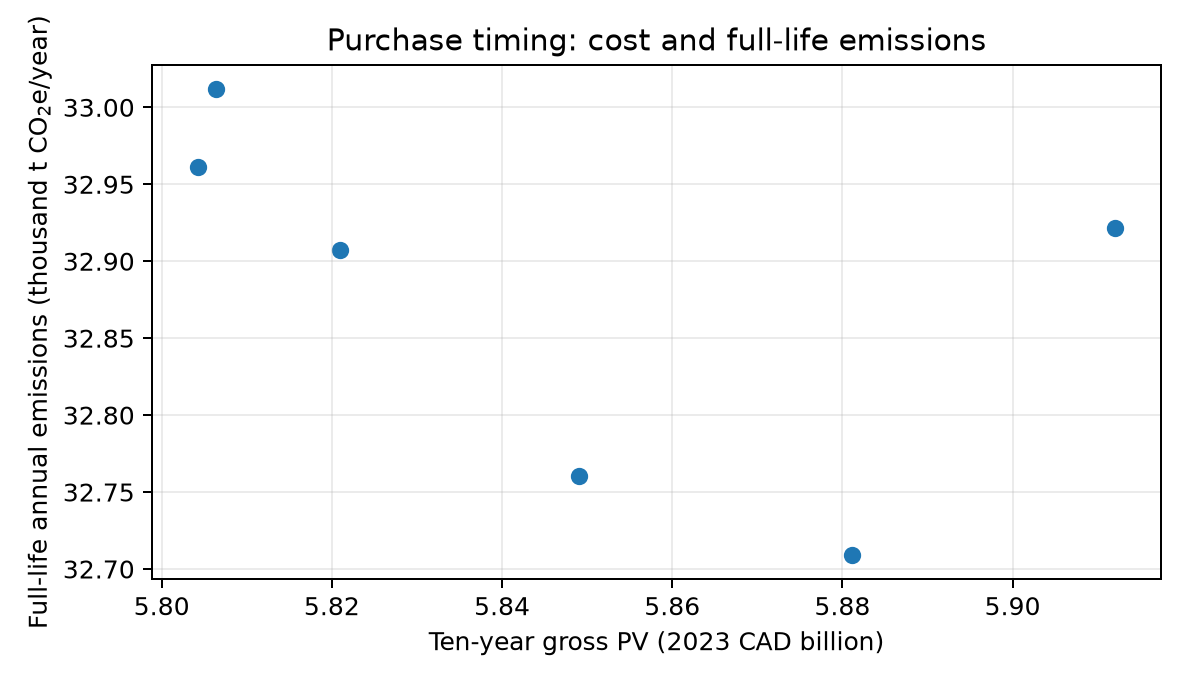
\includegraphics[width=0.78\linewidth]{generated/cost_lifecycle_tradeoff.png}
\caption{Discounted ten-year cost and annualized full-lifecycle emissions across the sampled purchase schedules.}
\end{figure}

\subsection{Cost, funding and emissions}

\begin{table}[htbp]
\centering
\caption{Canonical policy results. The full-lifecycle score is the main environmental comparison; the transition ledger is a separate near-term indicator.}
\begin{tabular}{lr}
\toprule
Indicator & Value\\\midrule
Gross ten-year cost, baseline & CAD \CV{finance.baseline_gross_pv_billion} bn\\
Gross ten-year cost, electric plan & CAD \CV{finance.plan_gross_pv_billion} bn\\
Conversion-fleet economic score, unsubsidized & \CV{finance.economic_score_pct}\%\\
Agency cost with 25\% capital support & CAD \CV{finance.agency_25_pv_billion} bn\\
Agency cost with 50\% capital support & CAD \CV{finance.agency_50_pv_billion} bn\\
Converted-fleet full-life environmental score & \CV{lifecycle.environment_score_pct}\%\\
Whole-fleet score with retained trolleys & \CV{lifecycle.whole_fleet_environment_score_pct}\%\\
2033 operating emission reduction & \CV{lifecycle.operation_reduction_pct}\%\\
2024--2033 transition emissions & \CV{lifecycle.transition_emissions_t} t CO$_2$e\\
\bottomrule
\end{tabular}
\end{table}

The headline recommendation is the portfolio with the lowest full-lifecycle emission inventory. The cost-minimizing alternative is reported beside it because it may delay some purchases without changing the final 2033 fleet. The difference between the two is the cost of accelerating environmental benefits; the transition ledger makes that trade-off visible without changing the environmental definition.

\FloatBarrier
\section{Three-city transfer and comparison}

The same equations are applied to Chicago and London with their public 2023 fleet registers. Vancouver uses the full dispatch model. Chicago uses its 1,875-bus fixed-route register with 25 inferred electric buses and the reported 73.08 million revenue bus-km. London uses the TfL 8,643-slot audit, including 950 electric positions, and its single- and double-deck body mix. The lower precision of the two comparator cities is a scale and technology-transfer test, not an alternative routing analysis.\cite{ctaprofile,ctaage,tflaudit}

\begin{table}[htbp]
\centering
\caption{Common-model transfer across the three metropolitan areas. Chicago and London are fleet-level comparison cases; Vancouver is the full service-feasible case.}
\begin{tabularx}{\linewidth}{@{}lrrr@{}}
\toprule
Quantity & Vancouver & Chicago & London\\
\midrule
2023 fixed-route fleet & 1,725 & 1,875 & 8,643\\
Existing electric stock & 280 & 25 & 950\\
Non-electric stock & 1,445 & 1,850 & 7,693\\
Annual service (million km) & 106.87 & 73.08 & \CV{london.service_million_km}\\
2033 non-electric remaining & 0 & 0 & 0\\
Peak annual EV deliveries & \CV{vancouver.peak_ev_deliveries} & \CV{chicago.peak_ev_deliveries} & \CV{london.peak_ev_deliveries}\\
Full-life emission score & \CV{vancouver.lifecycle_score} & \CV{chicago.lifecycle_score} & \CV{london.lifecycle_score}\\
Evidence level & full schedule & fleet register & fleet register\\
\bottomrule
\end{tabularx}
\end{table}

Vancouver's operational result provides the transfer ratios. We use its average annual distance per active bus, energy per service-km and vehicle mix to construct the two comparator scenarios. Chicago's larger standard-bus share and London's double-deck share are retained from their public registers. The table therefore tests whether a 2033 conversion is physically plausible at each city's observed fleet scale; it does not invent depot locations or route schedules for those cities.

The three cases share the same policy result: the electric fleet needs a concentrated build-and-purchase window, the peak delivery year is the binding procurement constraint, and financing must be secured before the first depot upgrade. Chicago's fleet is smaller but its age profile makes early replacement more expensive. London's double-deck concentration increases the charging and terminal-test problem, while its larger fleet moves the delivery bottleneck into a larger annual block.

\FloatBarrier
\section{Sensitivity and decision rules}

The recommendation is tested with five one-factor changes while the service schedule is held fixed: 10\% rather than 15\% reserve, full-new depot construction instead of retrofit-first, half-power charging, severe winter conditions, and a fossil-diesel baseline. The cost, full-life emission and peak-power outputs are reported together; the sensitivity table does not replace the central recommendation.

\begin{table}[htbp]
\centering
\caption{One-factor sensitivity of the canonical Vancouver recommendation. Values are filled from the generated canonical result.}
\begin{tabularx}{\linewidth}{@{}Xrrr@{}}
\toprule
Case & Economic score & Full-life environment & Peak power (MW)\\
\midrule
Central retrofit & \CV{sens.central.econ} & \CV{sens.central.env} & \CV{sens.central.power}\\
10\% reserve & \CV{sens.spare10.econ} & \CV{sens.spare10.env} & \CV{sens.spare10.power}\\
Full-new depot & \CV{sens.newbuild.econ} & \CV{sens.newbuild.env} & \CV{sens.newbuild.power}\\
Half-power charging & \CV{sens.slow.econ} & \CV{sens.slow.env} & \CV{sens.slow.power}\\
Severe winter & \CV{sens.winter.econ} & \CV{sens.winter.env} & \CV{sens.winter.power}\\
Fossil-diesel baseline & \CV{sens.fossil.econ} & \CV{sens.fossil.env} & \CV{sens.fossil.power}\\
\bottomrule
\end{tabularx}
\end{table}

The decision rules are straightforward. Release a site when its parking, charger positions and firm power are jointly available. Do not place a bus order against an uncommissioned site. Convert standard and articulated routes in the first waves because they deliver the largest early emission reduction with mature depot charging. Hold double-deck and small-shuttle purchases until the terminal-duty and winter tests pass. If the 50\% funding case is unavailable, keep the 2033 service target but slow the noncritical class conversions within the same total purchase envelope; the model does not recover affordability by cutting published trips.

\section{Conclusion}

The model produces a single service-preserving architecture for a 2033 all-electric fleet: a 119-day timetable becomes a verified set of electric duties, those duties become depot charging and reserve requirements, and the depot-by-class packages become a ten-year integer purchase roadmap. The plan retains the 275 trolleybuses and converts 1,445 conventional vehicles through a combination of retained-facility retrofits and targeted expansion.

The central result is not a comparison of an electric bus with an unchanged diesel bus. It compares the complete electric system with continued low-carbon renewal. The full-lifecycle score captures vehicle, battery and infrastructure manufacturing; the 2033 operating result captures the benefit that appears after commissioning. The former is the ecological decision metric; the latter is the near-term operational indicator.

The recommended action is to begin the depot and interconnection program immediately, publish a site release calendar, and buy only against committed charger capacity. The 50\% funding case should be presented to the funding partners as the implementation case. If the external contribution is smaller, the public authority must either extend the financing period or reduce the noncritical conversion rate; deleting scheduled service would fail the model's own feasibility condition.

\subsection*{Implementation controls}
\begin{itemize}
\item In 2024--25, complete depot design, utility interconnection applications and vehicle-platform selection; place no bus order before the associated site release is funded.
\item In 2026--29, complete the retrofit and expansion work in staged parcels, commissioning parking, charger ports and firm power as one acceptance package.
\item From 2030, release annual bus orders within the 650-vehicle ceiling; prioritise standard and articulated classes while double-deck and shuttle validation finishes.
\item At each quarterly review, reconcile delivered vehicles, commissioned power, winter energy and spare availability. A missed site date shifts the order release; it does not reduce service.
\end{itemize}

\clearpage
\appendix
\section{Technical appendix: evidence, calculations and verification}

\subsection{Evidence classes and assumptions}

\begin{table}[h]
\centering
\caption{Compact evidence ledger. The main text uses the same assumptions; audit detail remains in the repository.}
\begin{tabularx}{\linewidth}{@{}>{\raggedright\arraybackslash}p{0.18\linewidth}X>{\raggedright\arraybackslash}p{0.16\linewidth}@{}}
\toprule
Item & Use in the model & Status\\\midrule
GTFS timetable & Trips, times, directions, endpoints, 119-day patterns & Observed\\
Route load factors & Capacity class proxy, not vehicle identity & Derived\\
Fleet counts & 1,725 stock seed, 275 trolleys, five battery buses & Observed or assumed\\
Vehicle battery/charging & Class energy limits and release times & Observed specifications + planning values\\
Depot anchors & Pullout/pullin and site grouping & Assumed regional anchors\\
Electricity factor & Grid operating emissions & Public average\\
Vehicle and facility LCA factors & Production and construction burden & Published transfer factors\\
Prices and grants & Ten-year cash flow and funding cases & Public envelopes + transfer\\
\bottomrule
\end{tabularx}
\end{table}

\subsection{Reproducibility and checks}

The canonical run builds four scenario schedules (central, slow charging, severe winter and capacity stress) for the electric and conventional fleets. For each scenario it exports duties, trip assignments and the 119-day calendar. It then verifies:
\begin{itemize}
\item every source trip appears exactly once;
\item every assigned vehicle has sufficient route capacity;
\item every duty respects start time, transfer distance, return time and battery reserve;
\item every charge interval is below the charger power and does not collide with driving;
\item the last day's return is compatible with the first day's departure;
\item each annual package satisfies its depot parking and power requirement;
\item annual inventory balances, conventional stock reaches zero in 2033, and no conversion starts before its six-year construction window;
\item full-life manufacturing, facility and operating terms reconcile separately to the main and transition scores.
\end{itemize}

The canonical JSON file stores the input hashes, schedules, annual purchase ledgers, funding cases, three-city comparison and verification report. The manuscript tables are generated from that file rather than edited by hand. The old evidence audit scripts remain in the repository as supporting material.

\subsection{Technical notes}

The environmental score annualizes vehicle and station manufacturing over their engineering lives. It does not claim that manufacturing emissions occur physically after the factory gate; the transition ledger reports the year-by-year burden separately. End-of-life disposal of the initial conventional fleet is not credited as a benefit, and no local zero-carbon electricity certificate is assumed. The supply factor remains the provincial average.

The route model uses estimated road distance and depot anchors rather than surveyed land parcels. This is appropriate for a planning-level road map: it determines whether the timetable can be covered by a class-compatible fleet, and it produces the scale of charging and parking needed. Site acquisition and utility interconnection remain implementation decisions.

\clearpage
\addcontentsline{toc}{section}{Letter to a Metro Vancouver decision-maker}
\section*{Letter to a Metro Vancouver decision-maker}
\textbf{To:} TransLink Board and Mayors' Council\\
\textbf{Subject:} A service-preserving route to an all-electric fixed-route bus fleet by 2033

Dear decision-makers,

We recommend a 2033 fixed-route electric fleet that preserves all published trips. Our model assigns every non-trolley trip to a compatible electric duty, retains the 275 existing trolleybuses and checks each vehicle's route capacity, return trip, charging time and battery reserve. The recovered schedule contains 54,497 distinct trips and 495,198 trip instances across 25 service patterns. Under the central assumptions, the service-feasible battery fleet is \CV{schedule.fleet_with_spares} buses including a 15\% reserve, and the charging schedule requires \CV{schedule.required_peak_power_mw} MW of firm depot power.

Begin work in 2024. Retrofit the six existing depots first, release each site only after parking, charger positions and utility capacity are jointly commissioned, and add new parking only after the retained capacity is exhausted. Order no bus against an uncommissioned site. The first electric service begins after the six-year construction window, with annual deliveries constrained by a 650-bus procurement ceiling.

The complete plan costs CAD \CV{finance.plan_gross_pv_billion} billion in discounted resource terms, against CAD \CV{finance.baseline_gross_pv_billion} billion for continued low-carbon renewal. With 50\% capital support, the agency's ten-year payment falls to CAD \CV{finance.agency_50_pv_billion} billion. The full-lifecycle environmental score is \CV{lifecycle.environment_score_pct}\%, while the 2033 operating inventory falls by \CV{lifecycle.operation_reduction_pct}\%. These two results should be reported together: early construction creates a measurable one-time carbon liability, while the operating fleet produces a durable reduction thereafter.

We would make three commitments public: a 2024 design and interconnection start, an annual delivery schedule below the procurement ceiling, and a class-specific release test for double-deck and community-shuttle conversions. If external funding is below the 50\% case, extend the financing schedule or delay the hardest classes; do not reduce scheduled service to make the arithmetic look feasible. The service floor and the 2033 target are the two non-negotiable constraints.

Sincerely,\\
2023 HiMCM Team 00000

\newpage
\addcontentsline{toc}{section}{References}
\begin{thebibliography}{99}
\small
\raggedright
\setlength{\itemsep}{0.1em}
\bibitem{problem} 2023 HiMCM Problem B, user-provided problem statement.
\bibitem{gtfs2023} TransLink, \emph{GTFS static feed 23SEP\_20231020}, 4 September--31 December 2023, preserved at public Git commit \texttt{eb584b1}; route and arrival data used by permission of TransLink, \href{https://github.com/JaydenCWong/JAAM-project/tree/eb584b1108b0d582ae31c7db8e0d7e7b5ba1702b/backend/engine/translink_data}{Online mirror}.
\bibitem{vancouvercensus} Statistics Canada, \emph{Population and population growth rate of census metropolitan areas}, 2021 Census, released February 2022, \href{https://www150.statcan.gc.ca/n1/daily-quotidien/220209/t002a-eng.htm}{Online source}.
\bibitem{fleet2020} TransLink, \emph{Low Carbon Fleet Transition Plan}, 2020, \href{https://www.translink.ca/-/media/translink/documents/about-translink/policies/translink_low_carbon_fleet_transition_plan_2020_02_24.pdf}{Online source}.
\bibitem{playbook2024} TransLink, \emph{Zero Emissions Fleet Transition Plan} summary, Mayors' Council agenda, November 2024, \href{https://www.translink.ca/-/media/translink/documents/about-translink/governance-and-board/council-minutes-and-reports/2024/november/agenda--mayors-council--public-mtg--nov-28-2024.pdf}{Online source}.
\bibitem{guidelines2018} TransLink, \emph{Transit Service Guidelines}, June 2018, pp.~21, 49, \href{https://www.translink.ca/-/media/translink/documents/plans-and-projects/managing-the-transit-network/transit-oriented-communities/transit-services-guidelines-public-summary.pdf}{Online source}.
\bibitem{loadcsv} TransLink, 2023 TSPR direction peak-load CSV, \href{https://www.translink.ca/-/media/translink/documents/plans-and-projects/managing-the-transit-network/tspr/csv-data/2023/tspr2023_bus_peakload_yearlinedaytypeseasontimerangedirection.csv}{Online source}.
\bibitem{nova2021} Nova Bus, \emph{LFSe+ specification brochure}, battery, charging and passenger configurations, \href{https://us.novabus.com/wp-content/uploads/sites/2/2019/10/LFSe_brochure_march2021_EN.pdf}{Online source}.
\bibitem{newflyer2025} New Flyer, \emph{Xcelsior CHARGE NG}, product specifications, \href{https://www.newflyer.com/bus/xcelsior-charge-ng/}{Online source}.
\bibitem{winnipeg2023} City of Winnipeg, \emph{RFP 763-2023 Appendix A: 40-foot and 60-foot bus specification}, Table 1, 432/605 kWh and 90\% manufacturer usable capacity, \href{https://legacy.winnipeg.ca/finance/findata/matmgt/documents/2023/763-2023/763-2023_Appendix_A_Bus_Specification.pdf}{Online source}.
\bibitem{foothill2024} Foothill Transit, \emph{Executive Board agenda packet}, 26 January 2024, vehicle specification and contract p.~21, \href{https://www.foothilltransit.org/sites/default/files/2024-01/01-26-24_eb_agenda_packet.pdf}{Online source}.
\bibitem{endera2023} Endera, \emph{2023 all-electric shuttle with 150-kWh battery and fast charging}, \href{https://www.enderamotors.com/press-releases/endera-unveils-the-2023-all-electric-shuttle-model-with-extended-range-and-fast-charging-speeds}{Online source}.
\bibitem{corepm} Core Project Management, \emph{Marpole Transit Centre}, aggregate floor area approximately 800,000 ft$^2$, \href{https://corepm.ca/projects/marpole-transit-centre/}{Online source}.
\bibitem{june2023tech} TransLink, \emph{Zero Emissions Bus Fleet Technology Update}, Mayors' Council public agenda, June 2023, PDF pp.~28--29, \href{https://www.translink.ca/-/media/translink/documents/about-translink/governance-and-board/council-minutes-and-reports/2023/june/agenda_mayors_council_public_mtg_june_2023.pdf}{Online source}.
\bibitem{budget2025} TransLink, \emph{2025 Business Plan, Operating and Capital Budget Summary}, 2023 actual bus service p.~23 and capital-program details pp.~50--51, \href{https://www.translink.ca/-/media/translink/documents/about-translink/corporate-reports/business_plan/2025-business-plan-operating-and-capital-budget-summary.pdf}{Online source}.
\bibitem{bctariff2023} BC Hydro, \emph{Executed tariff pages, effective 1 April 2023}, RS1600/1640/1650 and RS1901, pp.~2-35--2-48 and 6-13, \href{https://www.bchydro.com/content/dam/BCHydro/customer-portal/documents/corporate/suppliers/transmission-scheduling/bulletins/2023/2023_08_03_BCUC_EXEC_TRFF_PGS.pdf}{Online source}.
\bibitem{cpi2025} Bank of Canada, \emph{Total CPI, series V41690973, 2019--2025}, \href{https://www.bankofcanada.ca/valet/observations/V41690973/json?start_date=2019-01-01&end_date=2025-12-31}{Online source}.
\bibitem{icct2024} A.~B. Rebou\c{c}as and A.~Cieplinski, \emph{Quantifying avoided greenhouse gas emissions by e-buses in Latin America: A simplified life-cycle assessment methodology}, ICCT Working Paper, 2024, \href{https://theicct.org/wp-content/uploads/2024/08/ID-118-\%E2\%80\%93-E-bus-radar_final2.pdf}{Online source}.
\bibitem{zhao2022} E.~Zhao, P.~D. Walker and N.~C. Surawski, \emph{Emissions life cycle assessment of diesel, hybrid and electric buses}, Proceedings of the Institution of Mechanical Engineers, Part D 236(6) (2022), \href{https://doi.org/10.1177/09544070211034318}{DOI}.
\bibitem{yeboah2025} D.~B. Yeboah and S.~Kaewunruen, \emph{Comparative lifecycle cost and sustainability assessments between very-light rail and bus-rapid transit}, Transportation Research Interdisciplinary Perspectives 32 (2025), 101529, \href{https://doi.org/10.1016/j.trip.2025.101529}{DOI}.
\bibitem{bcgrid} Government of British Columbia, \emph{Electricity emission factors}, \href{https://www2.gov.bc.ca/gov/content/environment/climate-change/data/electricity}{Online source}.
\bibitem{ctaprofile} Federal Transit Administration, \emph{2023 Annual Agency Profile: Chicago Transit Authority}, NTD ID 50066, pp.~1--2, \href{https://www.transit.dot.gov/sites/fta.dot.gov/files/transit_agency_profile_doc/2023/50066.pdf}{Online source}.
\bibitem{ctaage} U.S. Department of Transportation, \emph{NTD Vehicles: Age Distribution}, 2023 CTA records, NTD ID 50066, retrieved October 2026, \href{https://data.transportation.gov/d/6abt-uhgq}{Online source}.
\bibitem{tflaudit} TfL, \emph{Bus Fleet Audit, 31 March 2023}, \href{https://content.tfl.gov.uk/fleet-annual-audit-report-31-march-2023.pdf}{Online source}.
\bibitem{aicodex} OpenAI, \emph{Codex} (GPT-6), and \emph{deepseek-flash}, research, calculation and drafting assistance, October 2026. See the appended Report on Use of AI, with the request log in \nolinkurl{materials/research/ai_query_log.md} and artifact map in \nolinkurl{materials/research/ai_use_report.md}.
\end{thebibliography}

\newpage
\section*{Report on Use of AI}
\textbf{Tools.} OpenAI Codex (GPT-6) and deepseek-flash were used in October 2026 for research planning, source discovery, code implementation, numerical checks and LaTeX drafting. No 2023 HiMCM solution paper was requested or used.\cite{aicodex}

\textbf{Work products.} The study includes repository code for timetable processing, duty generation, charging checks, a mixed-integer transition model, a full-life environmental ledger, three-city parameter comparisons and manuscript generation. The query log and artifact map are retained in the project repository.

\textbf{Verification.} The generated schedule and annual plan are checked by independent trip, energy, cycle, inventory and accounting tests. The human team should review the submitted narrative and verify every cited public fact before submission.

\end{document}
